\section{Data reduction}

\begin{frame}{Data Reduction (I)}
	\begin{itemize}
		\item \textbf{What is data reduction?}\\
		      \begin{itemize}
			      \item Obtain a reduced representation of the data set that is much
			            smaller in volume but yet produces the same (or almost the same)
			            results.
		      \end{itemize}
		\item \textbf{Why data reduction?}\\
		      \begin{itemize}
			      \item A database/data warehouse may store terabytes of data.
			      \item Complex data analysis may take a very long time to run on the
			            complete data set.
		      \end{itemize}
		\item \textbf{Data reduction strategies:}
		      \begin{itemize}
			      \item Dimensionality reduction, i.e. remove unimportant attributes.
			            \begin{itemize}
				            \item Wavelet transforms.
				            \item Principal component analysis.
				            \item Attribute subset selection or attribute creation.
			            \end{itemize}
		      \end{itemize}
	\end{itemize}
\end{frame}

\begin{frame}{Data Reduction (II)}
	\begin{itemize}
		\item \textbf{Data reduction strategies (continued):}
		      \begin{itemize}
			      \item Numerosity reduction:
			            \begin{itemize}
				            \item Regression and log-linear models.
				            \item Histograms, clustering and sampling.
				            \item Data cube aggregation.
			            \end{itemize}
			      \item Data compression.
		      \end{itemize}
	\end{itemize}
\end{frame}

\begin{frame}{Data Reduction (I): Dimensionality Reduction}
	\begin{itemize}
		\item \textbf{Curse of dimensionality:}
		      \begin{itemize}
			      \item When dimensionality increases data becomes increasingly
			            sparse.
			      \item Density and distance between points become less meaningful.
			      \item The possible combinations of subspaces will grow
			            exponentially.
		      \end{itemize}
		\item \textbf{Dimensionality reduction:}
		      \begin{itemize}
			      \item Avoid the curse of dimensionality.
			      \item Help eliminate irrelevant features and reduce noise.
			      \item Reduce time and space required in data mining.
			      \item Allow easier visualization.
		      \end{itemize}
		\item \textbf{Dimensionality-reduction techniques:}
		      \begin{itemize}
			      \item Wavelet transforms.
			      \item Principal component analysis.
			      \item Supervised and nonlinear techniques (e.g. feature selection).
		      \end{itemize}
	\end{itemize}
\end{frame}

\begin{frame}{Wavelet Transform (I)}
	\begin{minipage}[t]{0.55\textwidth}
		\begin{itemize}
			\item \textbf{Decomposes a signal into different frequency
				      subbands.}\\
			      Applicable to $n$-dimensional signals.
			\item Data transformed to preserve relative distance between
			      objects at different levels of resolution.
			\item Allow natural clusters to become more distinguishable.
			\item Used for image compression.
		\end{itemize}
	\end{minipage}\hspace{1cm}
	\begin{minipage}[t]{0.30\textwidth}
		\raisebox{\dimexpr-\height+\ht\strutbox\relax}{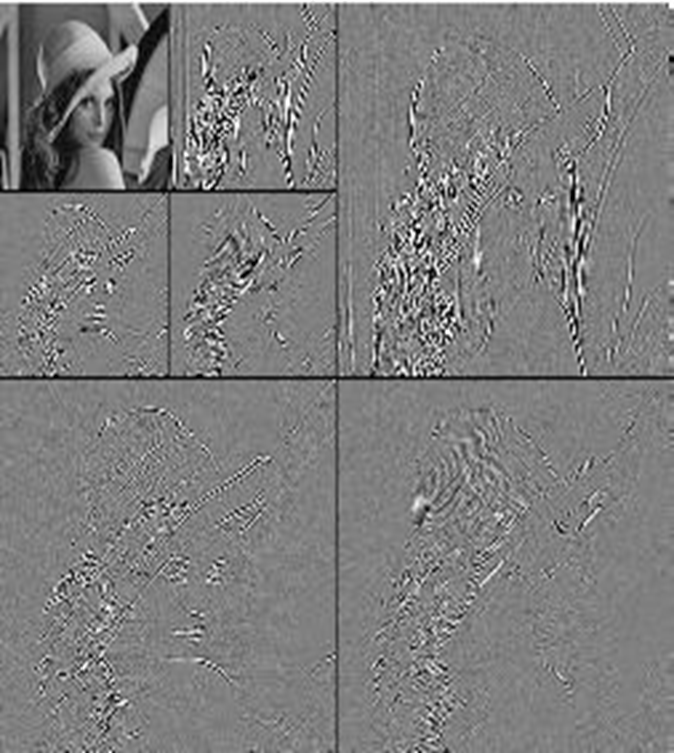
\includegraphics[width=5cm]{img/wavelettransform.png}}
	\end{minipage}
\end{frame}

\begin{frame}{Wavelet Transform (II)}
	\begin{itemize}
		\item \textbf{Discrete wavelet transform:}\\
		      Transforms a vector $X$ into a different vector $X'$ of wavelet
		      coefficients with the same length.
		\item \textbf{Compressed approximation:}\\
		      Store only a small fraction of the strongest of the wavelet
		      coefficients.
		\item \textbf{Similar to discrete fourier transform, but better lossy
			      compression, localized in space.}
		\item \textbf{Method:}
		      \begin{itemize}
			      \item The length of the vector must be an integer power of $2$
			            (padding with $0$'s if necessary).
			      \item Each transform has two functions: smoothing and difference.
			      \item Applied to pairs of data, resulting in two sets of data with
			            half the length.
			      \item The two functions are applied recursively until reaching the
			            desired length.
		      \end{itemize}
	\end{itemize}
\end{frame}

\begin{frame}{Example: Wavelet Transform (I)}
	\begin{itemize}
		\item \textbf{Initial vector:}
		      \begin{itemize}
			      \item $X = (2,2,0,2,3,5,4,4)$
		      \end{itemize}
		\item \textbf{First step:}
		      \begin{itemize}
			      \item $(2,2) \rightarrow \text{Average: } 2, \text{Weighted
					            difference: } 0$
			      \item $(0,2) \rightarrow \text{Average: } 1, \text{Weighted
					            difference: } -1$
			      \item $(3,5) \rightarrow \text{Average: } 4, \text{Weighted
					            difference: } -1$
			      \item $(4,4) \rightarrow \text{Average: } 4, \text{Weighted
					            difference: } 0$
			      \item $A_1=(2,1,4,4), D_1=(0,-1,-1,0)$
		      \end{itemize}
		\item \textbf{Second step:}
		      \begin{itemize}
			      \item $(2,1) \rightarrow \text{Average: } 1.5, \text{Weighted
					            difference: } 0.5$
			      \item $(4,4) \rightarrow \text{Average: } 4, \text{Weighted
					            difference: } 0$
			      \item $A_2=(1.5,4), D_2=(0.5,0)$
		      \end{itemize}
	\end{itemize}
\end{frame}

\begin{frame}{Example: Wavelet Transform (II)}
	\begin{itemize}
		\item \textbf{Third step:}
		      \begin{itemize}
			      \item $(1.5,4) \rightarrow \text{Average: } 2.75, \text{Weighted
					            difference: } -1.25$
			      \item $A_3=(2.75), D_3=(-1.25)$
		      \end{itemize}
		\item \textbf{Resulting vector:}
		      \begin{itemize}
			      \item $X' = (2.75,-1.25,0.5,0,0,-1,-1,0)$
		      \end{itemize}
		\item \textbf{Possible compression:}\\
		      \begin{itemize}
			      \item Small detail coefficients ($D_{1,2,3}$) can be replaced by
			            $0$'s,
			            while retaining significant coefficients.
		      \end{itemize}
	\end{itemize}
	\vspace{0.2cm}
	\centering
	\begin{tabular}{|c|c|c|}
		\hline
		\text{Resolution} & \text{Averages}     & \text{Detail coefficients}
		\\\hline
		$8$               & $(2,2,0,2,3,5,4,4)$ & -
		\\\hline
		$4$               & $(2,1,4,4)$         & $(0,-1,-1,0)$
		\\\hline
		$2$               & $(1.5,4)$           & $(0.5,0)$
		\\\hline
		$1$               & $(2.75)$            & $(-1.25)$
		\\\hline
	\end{tabular}
\end{frame}

\begin{frame}{Why Wavelet Transform?}
	\begin{itemize}
		\item \textbf{Hat-shaped filters:}
		      \begin{itemize}
			      \item Emphasize region where points cluster.
			      \item Suppress weaker information in their boundaries.
		      \end{itemize}
		\item \textbf{Effective removal of outliers:}
		      \begin{itemize}
			      \item Insensitive to noise, insensitive to input order.
		      \end{itemize}
		\item \textbf{Multi-resolution:}
		      \begin{itemize}
			      \item Detect arbitrary shaped clusters at different scales.
		      \end{itemize}
		\item \textbf{Efficient:} Complexity $\mathcal{O}(N)$.
	\end{itemize}
\end{frame}

\begin{frame}{Principal Component Analysis (PCA)}
	\begin{itemize}
		\item \textbf{Main idea:}
		      \begin{itemize}
			      \item Given a data set with $n$ dimensions.
			      \item Find $k \leq n$ orthogonal vectors that capture the largest
			            amount of data.
			      \item Works only for numeric data.
		      \end{itemize}
		\item \textbf{Example data set:}
		      \begin{itemize}
			      \item Used on the next few slides to explain the steps of a PCA:
		      \end{itemize}
		      \vspace{3mm}
		      \centering
		      \begin{tabular}{|c|c|c|}
			      \hline
			      $d_1$ & $d_2$ & $d_3$
			      \\\hline
			      $23$  & $6$   & $1$
			      \\\hline
			      $9$   & $9$   & $5$
			      \\\hline
			      $17$  & $5$   & $1$
			      \\\hline
			      $3$   & $6$   & $1$
			      \\\hline
		      \end{tabular}
	\end{itemize}
\end{frame}

\begin{frame}{Principal Component Analysis - 1. Step: Standardization (I)}
	\begin{itemize}
		\item \textbf{Procedure:}
		      \begin{itemize}
			      \item Each value $x$ within a dimension $d_n$ is standardized with
			            the help of the mean ($\mu_{d_n}$) and standard deviation
			            ($\sigma_{d_n}$) of $d_n$:
			            \begin{align*}
				            x' = \frac{x - \mu_{d_n}}{\sigma_{d_n}}
			            \end{align*}
		      \end{itemize}
		\item \textbf{Reason:}
		      \begin{itemize}
			      \item Each dimension should be considered equally in the analysis.
			      \item Dimensions with a wider range of	values would dominate
			            without this step.
		      \end{itemize}
	\end{itemize}
\end{frame}

\begin{frame}{Principal Component Analysis - 1. Step: Standardization (II)}
	\begin{itemize}
		\item \textbf{Example:}
		      \begin{itemize}
			      \item Mean and standard deviation per dimension: \\
			            \vspace{3mm}
			            \begin{center}
				            \centering
				            \begin{tabular}{|l|c|c|c|}
					            \hline
					                     & $d_1$     & $d_2$     & $d_3$
					            \\\hline
					            $\mu$    & $13$      & $6.5$     & $3$
					            \\\hline
					            $\sigma$ & $8.79394$ & $1.73205$ &
					            $2$
					            \\\hline
				            \end{tabular}
			            \end{center}
			            \vspace{3mm}
			      \item Standardized data set: \\
			            \vspace{3mm}
			            \begin{center}
				            \centering
				            \begin{tabular}{|c|c|c|}
					            \hline
					            $d_1$      & $d_2$      & $d_3$
					            \\\hline
					            $+1,13715$ & $-0,28868$ & $-1$
					            \\\hline
					            $-0,45486$ & $+1,44338$ & $+1$
					            \\\hline
					            $+0,45486$ & $-0,86603$ & $-1$
					            \\\hline
					            $-1,13715$ & $-0,28868$ & $-1$
					            \\\hline
				            \end{tabular}
			            \end{center}
		      \end{itemize}
	\end{itemize}
\end{frame}

\begin{frame}{Principal Component Analysis - 2. Step: Covariance Matrix (I)}
	\begin{itemize}
		\item \textbf{Procedure:}
		      \begin{itemize}
			      \item A n x n covariance matrix is generated that contains the
			            covariance between each possible attribute pairing. When the
			            dimensions are compared with themselves, the variance always
			            replaces the covariance:
			            \begin{align*}
				            \begin{bmatrix}
					            \text{Var}(d_1)      & ... & \text{Cov}(d_1, d_n) \\
					            ...                  & ... & ...                  \\
					            \text{Cov}(d_n, d_1) & ... & \text{Var}(d_n)      \\
				            \end{bmatrix}
			            \end{align*}
		      \end{itemize}
		\item \textbf{Reason:}
		      \begin{itemize}
			      \item Dimensions that are highly correlated contain redundant
			            information.
			      \item This step helps to identify these correlations.
		      \end{itemize}
	\end{itemize}
\end{frame}

\begin{frame}{Principal Component Analysis - 2. Step: Covariance Matrix (II)}
	\begin{itemize}
		\item \textbf{Example:}
		      \begin{itemize}
			      \item The 3 x 3 covariance matrix of our example: \\
			            \vspace{3mm}
			            \begin{center}
				            \centering
				            \begin{tabular}{|l|c|c|c|}
					            \hline
					                  & $d_1$      & $d_2$      & $d_3$
					            \\\hline
					            $d_1$ & $+0.75000$ & $-0.35015$ &
					            $-0.30324$
					            \\\hline
					            $d_2$ & $-0.35015$ & $+0.75000$ &
					            $+0.96225$
					            \\\hline
					            $d_3$ & $-0.30324$ & $+0.96225$ &
					            $+0.75000$
					            \\\hline
				            \end{tabular}
			            \end{center}
		      \end{itemize}
	\end{itemize}
\end{frame}

\begin{frame}{Principal Component Analysis - 3. Step: Eigenvalues (I)}
	\begin{itemize}
		\item \textbf{Procedure:}
		      \begin{itemize}
			      \item The eigenvectors and eigenvalues of the covariance matrix
			            ($C$) are computed by solving the following equation:
			            \begin{align*}
				            C \nu = \lambda \nu
			            \end{align*}
			      \item If an n digit vector $\nu$ satisfies this equation for a
			            $\lambda \in \mathbb{R}$, then $\nu$ is called an eigenvector with
			            associated eigenvalue $\lambda$
		      \end{itemize}
		\item \textbf{Reason:}
		      \begin{itemize}
			      \item The determined eigenvectors are called \textbf{prinicipal
				            components} of the dataset. The eigenvalues indicate which of these
			            prinicipal components has which importance for the significance of
			            the dataset.
			      \item By sorting the eigenvectors in descending order according to
			            their eigenvalues, the prinicipal components that contain the most
			            information can be identified.
		      \end{itemize}
	\end{itemize}
\end{frame}

\begin{frame}{Principal Component Analysis - 3. Step: Eigenvalues (II)}
	\begin{itemize}
		\item \textbf{Example:}
		      \begin{itemize}
			      \item Eigenvalues and eigenvectors in our example: \\
			            \begin{align*}
				            \lambda_1 = -0,21354,
				            \nu_1 = \begin{bmatrix} -0,05553 \\ -1,01884 \\ +1 \end{bmatrix}
				            \\
				            \lambda_2 = +0,56530,
				            \nu_2 = \begin{bmatrix} +3,17456 \\ +0,80847 \\ +1 \end{bmatrix}
				            \\
				            \lambda_3 = +1,89823,
				            \nu_3 = \begin{bmatrix} -0,57292 \\ +1,01273 \\ +1 \end{bmatrix}
			            \end{align*}
			      \item Sorting these three eigenvectors by their significance, we
			            arrive at the order $\nu_3$, $\nu_2$, $\nu_1$
		      \end{itemize}
	\end{itemize}
\end{frame}

\begin{frame}{Principal Component Analysis - 4. Step: Feature matrix (I)}
	\begin{itemize}
		\item \textbf{Procedure:}
		      \begin{itemize}
			      \item The top N eigenvectors are selected to create a feature
			            matrix from them.
			      \item There is no fixed rule exactly how many eigenvectors should
			            be selected.
			      \item The dimensionality reduction is larger the
			            fewer eigenvectors are chosen.
			      \item The information loss increases with each eigenvector that is
			            discarded.
		      \end{itemize}
		\item \textbf{Reason:}
		      \begin{itemize}
			      \item It must be considered carefully how much information can be
			            given up in favor of dimensionality reduction.
		      \end{itemize}
	\end{itemize}
\end{frame}

\begin{frame}{Principal Component Analysis - 4. Step: Feature matrix (II)}
	\begin{itemize}
		\item \textbf{Example:}
		      \begin{itemize}
			      \item In our example $\nu_3$ carries approx. $71\%$ of the
			            information: \\
			            \begin{align*}
				            \frac{1,89823}{1,89823+0,5653+0,21354} = 0,70906
			            \end{align*}
			      \item It might be interesting to keep only the eigenvector $\nu_3$
			            and discard the other two eigenvectors. Our feature matrix
			            therefore looks as follows:
			            \begin{align*}
				            \begin{bmatrix} -0,57292 \\ +1,01273 \\ +1\end{bmatrix}
			            \end{align*}
		      \end{itemize}
	\end{itemize}
\end{frame}

\begin{frame}{Principal Component Analysis - 5. Step: Transformation (I)}
	\begin{itemize}
		\item \textbf{Procedure:}
		      \begin{itemize}
			      \item The original data set ($D$) gets multiplied with the feature
			            matrix ($F$), to create a new data set ($N$) with lower
			            dimensionality:
			            \begin{align*}
				            N = D \cdot F
			            \end{align*}
		      \end{itemize}
		\item \textbf{Reason:}
		      \begin{itemize}
			      \item This step applies the dimensionality reduction to each tuple.
			      \item The PCA is completed with this step.
		      \end{itemize}
	\end{itemize}
\end{frame}

\begin{frame}{Principal Component Analysis - 5. Step: Transformation (II)}
	\begin{itemize}
		\item \textbf{Example:}
		      \begin{itemize}
			      \item Our dataset after the transformation and with the PCA
			            completed looks like this: \\
			            \begin{align*}
				            \begin{bmatrix} -6,10078 \\ +8,95829 \\ -3,67599 \\ +5,35762
				            \end{bmatrix}
			            \end{align*}
			      \item It is to be expected that this dataset still contains about
			            $71\%$ of its original information, which can be
			            further used for data mining, while having to deal with
			            a lot less dimensions.
		      \end{itemize}
	\end{itemize}
\end{frame}

\begin{frame}{Attribute-subset Selection}
	\begin{itemize}
		\item \textbf{Another way to reduce dimensionality of data.}
		      \item\textbf{\color{airforceblue}Redundant attributes:}
		      \begin{itemize}
			      \item Duplicate much or all of the information contained in other
			            attributes.
			            \begin{itemize}
				            \item E.g. purchase price of a product and the amount of sales
				                  tax paid.
			            \end{itemize}
		      \end{itemize}
		\item \textbf{\color{airforceblue}Irrelevant attributes:}
		      \begin{itemize}
			      \item contain no information that is useful for the data-mining
			            task at hand.
			            \begin{itemize}
				            \item E.g. students' ID is often irrelevant to the task of
				                  predicting students' GPA.
			            \end{itemize}
		      \end{itemize}
	\end{itemize}
\end{frame}

\begin{frame}{Heuristic Search in Attribute Selection}
	\begin{itemize}
		\item \textbf{There are $2^d$ possible attribute combinations of $d$
			      attributes.}
		      \item\textbf{\color{airforceblue}Typical heuristic attribute-selection
			      methods:}
		      \begin{itemize}
			      \item Best single attribute under the attribute-independence
			            assumption: \\ choose by significance tests (e.g. t-test, see
			            Chapter 6).
			      \item Best step-wise feature selection:
			            \begin{itemize}
				            \item The best single attribute is picked first.
				            \item Then next best attribute condition to the first \ldots
			            \end{itemize}
		      \end{itemize}
		\item \textbf{\color{airforceblue}Step-wise attribute elimination:}
		      \begin{itemize}
			      \item Repeatedly eliminate the worst attribute.
		      \end{itemize}
		\item Best combined attribute selection and elimination.
		\item Optimal branch and bound:
		      \begin{itemize}
			      \item Use attribute elimination and backtracking.
		      \end{itemize}
	\end{itemize}
\end{frame}

\begin{frame}{Attribute Creation (Feature Generation)}
	\begin{itemize}
		\item \textbf{Create new attributes (features) that can capture the
			      important information in a data set more effectively than the original
			      ones.}
		\item \textbf{Three general methodologies:}
		      \begin{itemize}
			      \item Attribute extraction.
			            \begin{itemize}
				            \item Domain-specific.
			            \end{itemize}
			      \item Mapping data to new space (see: data reduction).
			            \begin{itemize}
				            \item E.g. Fourier transformation, wavelet transformation,
				                  manifold approaches (not covered).
			            \end{itemize}
			      \item Attribute construction:
			            \begin{itemize}
				            \item Combining features (see: discriminative frequent patterns
				                  in Chapter 5).
				            \item Data discretization.
			            \end{itemize}
		      \end{itemize}
	\end{itemize}
\end{frame}

\begin{frame}{Data Reduction (II): Numerosity Reduction}
	\begin{itemize}
		\item \textbf{Reduce data volume by choosing alternative,
			      {\color{airforceblue}smaller} forms of data representation.}
		\item \textbf{{\color{airforceblue}Parametric} methods (e.g.,
			      regression):}
		      \begin{itemize}
			      \item Assume the data fits some
			            \textbf{{\color{airforceblue}model}} (e.g. a function).
			      \item Estimate model parameters.
			      \item Store only the parameters.
			      \item Discard the data (except possible outliers):
			            \begin{itemize}
				            \item Ex. log-linear models obtain value at a point in
				                  $m$-dimensional space as the product of appropriate marginal
				                  subspaces.
			            \end{itemize}
		      \end{itemize}
		\item \textbf{{\color{airforceblue}Non-parametric} methods:}
		      \begin{itemize}
			      \item Do not assume models.
			      \item Major families: histograms, clustering, sampling, \ldots
		      \end{itemize}
	\end{itemize}
\end{frame}

\begin{frame}{Histogram Analysis}
	\begin{itemize}
		\item \textbf{Divide data into buckets and store average (sum) of each
			      bucket.}
		\item \textbf{Partitioning rules:}
		      \begin{itemize}
			      \item Equal-width: equal bucket range.
			      \item Equal-frequency (or equal-depth).
		      \end{itemize}
	\end{itemize}
	\centering
	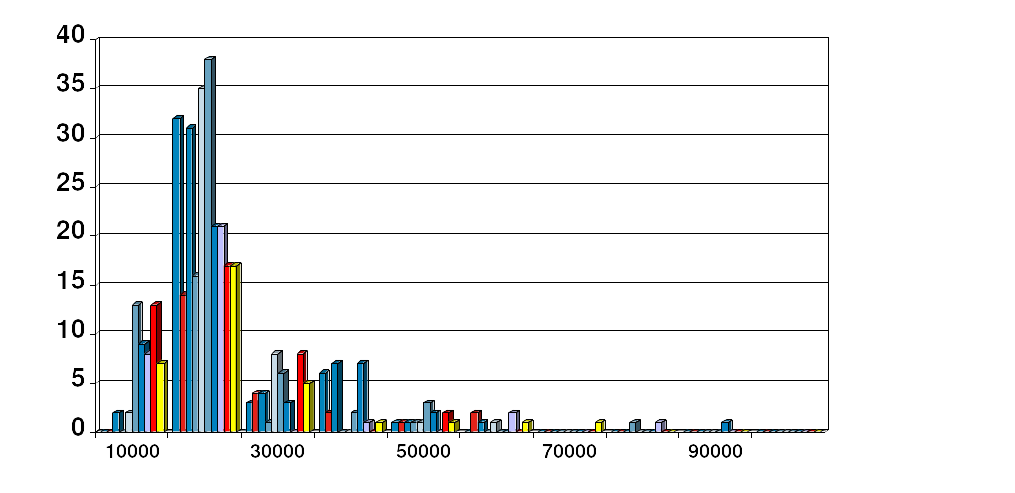
\includegraphics[width=9.5cm]{img/histogram.png}
\end{frame}

\begin{frame}{Clustering}
	\begin{itemize}
		\item \textbf{Partition data set into clusters based on similarity and
			      store cluster representation (e.g., centroid and diameter) only.}
		      \begin{itemize}
			      \item Can be very effective if data points are close to each other
			            under a certain norm and choice of space.
			      \item Can have hierarchical clustering and be stored in
			            multidimensional index-tree structures.
			      \item There are many choices of clustering algorithms.
			      \item Cluster analysis will be studied in depth in Chapter 7.
		      \end{itemize}
	\end{itemize}
\end{frame}

\begin{frame}{Sampling}
	\begin{itemize}
		\item \textbf{Obtain a small sample $x$ to represent the whole data set
			      $X$.}
		\item \textbf{Allow a mining algorithm to run in complexity \\ that is
			      potentially sub-linear to the size of the data.}
		\item \textbf{Key principle: Choose a
				      {\color{airforceblue}representative} subset of the data.}
		      \begin{itemize}
			      \item Simple random sampling may have very poor performance in the
			            presence of skew.
			      \item Develop adaptive sampling methods, e.g. stratified sampling.
		      \end{itemize}
		\item \textbf{Note: Sampling may not reduce database I/Os.}
		      \begin{itemize}
			      \item One page at a time.
		      \end{itemize}
	\end{itemize}
\end{frame}

\begin{frame}{Types of Sampling}
	\begin{itemize}
		\item \textbf{Simple random sampling.}
		      \begin{itemize}
			      \item There is an equal probability of selecting any particular
			            item.
		      \end{itemize}
		\item \textbf{Sampling without repetition.}
		      \begin{itemize}
			      \item Once an object is selected, it is removed from the population.
		      \end{itemize}
		\item \textbf{Sampling with repetition.}
		      \begin{itemize}
			      \item A selected object is not removed from the population.
		      \end{itemize}
		\item \textbf{Stratified sampling:}
		      \begin{itemize}
			      \item Partition the data set and draw samples from each partition:
			            Proportionally, i.e. approximately the same percentage of the data.
			      \item Used in conjunction with skewed data.
		      \end{itemize}
	\end{itemize}
\end{frame}

\begin{frame}{Data-cube Aggregation}
	\begin{itemize}
		\item \textbf{The lowest level of a data cube (base cuboid).}
		      \begin{itemize}
			      \item The aggregated data for an \textbf{individual entity of
				            interest}.
			      \item E.g. a customer in a phone-calling data warehouse.
			      \item Number of calls per hour, day, or week.
		      \end{itemize}
		\item \textbf{Multiple levels of aggregation in data cubes.}
		      \begin{itemize}
			      \item Further reduce the size of data to deal with.
		      \end{itemize}
		\item \textbf{Reference appropriate levels.}
		      \begin{itemize}
			      \item Use the smallest representation that is enough to solve
			            the task.
		      \end{itemize}
		\item \textbf{Queries regarding aggregated information should be
			      answered using the data cube, if possible.}
	\end{itemize}
\end{frame}

\begin{frame}{Data Reduction (III): Data Compression}
	\begin{itemize}
		\item \textbf{String compression.}
		      \begin{itemize}
			      \item There are extensive theories and well-tuned algorithms.
			      \item Typically lossless, but only limited manipulation is possible
			            without expansion.
		      \end{itemize}
		\item \textbf{Audio/video compression.}
		      \begin{itemize}
			      \item Typically lossy compression, with progressive refinement.
			      \item Sometimes small fragments of signal can be reconstructed
			            without reconstructing the whole.
		      \end{itemize}
		\item \textbf{Time sequence is not audio.}
		      \begin{itemize}
			      \item Typically short and varies slowly with time.
		      \end{itemize}
		\item \textbf{Dimensionality and numerosity reduction may also be
			      considered as forms of data compression.}
	\end{itemize}
\end{frame}
